\documentclass{beamer}
%
% Choose how your presentation looks.
%
% For more themes, color themes and font themes, see:
% http://deic.uab.es/~iblanes/beamer_gallery/index_by_theme.html
%
\mode<presentation>
{
  \usetheme{default}      % or try Darmstadt, Madrid, Warsaw, ...
  \usecolortheme{default} % or try albatross, beaver, crane, ...
  \usefonttheme{default}  % or try serif, structurebold, ...
  \setbeamertemplate{navigation symbols}{}
  \setbeamertemplate{caption}[numbered]
}

\usepackage[english]{babel}
\usepackage[utf8]{inputenc}
\usepackage[T1]{fontenc}

\title[CACTI]{Presentation for CACTI: Captcha Avoidance via Client-side TEE Integration}
\author{Bhanuj Gandhi$^{(2022201068)}$\\ Aakash Tripathi$^{(2022201053)}$\\ Jatin Sharma$^{(2022201023)}$}
\institute{International Institute of Information Technology, Hyderabad}
\date{March 31, 2023}

\begin{document}

\begin{frame}
  \titlepage
\end{frame}

% Uncomment these lines for an automatically generated outline.
%\begin{frame}{Outline}
%  \tableofcontents
%\end{frame}

\section{Introduction}

\begin{frame}{Introduction}

\begin{itemize}
  \item CAPTCHA stands for Completely Automated Public Turing test to tell Computers and Humans Apart.
  \item These are some tests which are very easily solvable by humans, but relatively very hard for machines to solve. CAPTCHAS are used to verify that a user is human and not a computer program attempting to perform automated tasks or spam.
  \item CAPTCHAs involve solving some test that require some visual or audio tasks. The most popular form of CAPTCHAs used are visual CAPTCHA.

\end{itemize}

\begin{figure}
	
\includegraphics[scale=0.5]{img1.png}
	
\includegraphics[scale=0.5]{img2.jpg}
	\caption{reCAPCTHA [1]}
\end{figure}

\end{frame}

\begin{frame}{Downside of CAPTCHA}

	\begin{itemize}
		\item Since CAPTCHA involves some audio/visual tasks, people with hearing impairment, color blindness or low vision find it difficult to solve.
		\item Solving them can be sometimes frustrating for the users. Some leave the website or the service instead of solving the puzzle.
		\item CAPTCHAs can also be solved with a reasonable accuracy using machine learning algorithms. Methods proposed by Gao Y. et. al[2] and Hossen M. et. al. [3] proves to solve the puzzles easily.
		\item CAPTCHA also have some major privacy concerns [4].
		\item Also there are entities called ‘CAPTCHA farms’ which employee people to solve them and pay them money based on number of CAPTCHAs they solve.
	\end{itemize}

\end{frame}

\begin{frame}{What the paper has to offer?}
	\begin{itemize}
		\item The paper does not aims at eliminating CAPTCHAs. It just aims at avoiding them.

		\item The paper aims at identifying the legitimate users from all the incoming requests to a service. These legitimate users will then directly be allowed to proceed without solving CAPTCHA.

		\item The users who are illegitimate or suspected to be illegitimate still need to solve the CAPTCHA puzzle.
	\end{itemize}
\end{frame}

\begin{frame}{CACTI-Captcha Avoidance via client side TEE Integration}
	\begin{itemize}
		\item The authors propose a mechanism called CACTI [5], which will use of cryptographic proofs called ‘rate proofs’ which is a measure of activity of the user. If this rate proof is below a threshold, then the user can be identified as a legitimate user.
		\item Using client-side TEEs, CACTI [5] allows legitimate clients to generate unforgeable rate-proofs demonstrating how frequently they have performed specific actions.
		\item Upon performing a sensitive action, like creating an account or booking a ticket, the server using these rate proofs can verify that the user is indeed legitimate and hence can allow it to proceed without CAPTCHA.
	\end{itemize}
\end{frame}

\begin{frame}{Background-Trusted Execution Environment(TEE)}
	Trusted Execution Environments (TEEs) are secure areas within a device's hardware that provide a trusted environment for executing code and processing data. TEEs are designed to provide a secure and isolated execution environment that is separate from the main operating system (OS) and other applications running on the device.

	TEE provides
	\begin{itemize}
		\item Isolated execution(“Enclave”)
		\item Persistent storage
		\item Remote attestation
	\end{itemize}

	TEE Drawbacks
	\begin{itemize}
		\item Limited storage
	\end{itemize}
\end{frame}

\begin{frame}{Background-Group signature schemes}
	\begin{itemize}
		\item Group signature schemes enable anonymous signing of a message on behalf of a group while ensuring the message's authenticity and integrity.
		\item Each group member has a secret key and corresponding public key, while the group has a public key known to everyone.
		\item To sign a message, a group member uses their secret key to generate a signature tied to the group's public key, providing anonymity to the signer while allowing anyone to verify the signature using the group's public key.
		\item Despite these concerns, group signature schemes have the potential to provide a valuable solution to certain authentication problems.
		\item This approach offers advantages such as openability, anonymity, and unlinkability. Remote attestation relies on group signatures, which consist of a shared public key and multiple private keys.
	\end{itemize}
\end{frame}

\begin{frame}{Captcha Avoidance using TEEs}
	\begin{itemize}
	\item Suppose a client tries to login onto a website. To identify the legitimacy of a user, the server sends a threshold starting time (ts), a new time stamp(t), a value k, its private key and its signature. It asks the user “if there are no more than k timestamp since ts, store t and provide a rate proof”.
	\item Basically in this step, the client is able to know the value of the threshold (k) corresponding to that website.
	\item If client’s activity is less than k, it will not receive any CAPTCHA, else, it will receive a CAPTCHA on the suspicion of an illegitimate user by the server.
	\item To bypass this, the bot just has to access the website once to know the value of threshold of that website.
	\item Then it just has to ensure that it needs to limit its activity below the value k to not receive the CAPCHA and bypass the security check.
	\end{itemize}
\end{frame}

\begin{frame}{Producing rate proofs}
	A new concept of ‘Rate Proofs’ is introduced in this paper. Rate proofs are cryptographic proofs that give information regarding the rate of performing sensitive actions by the client (such as clicking mouse, scrolling down etc). Rate proofs are generated on the client-side's Trusted Execution Environment. These rate proofs are an alternative way of proving legitimacy instead of solving a CAPTCHA which can be frustrating for many users In order to produce rate proofs, the client provides list and timestamps information to TEE. TEE then does hash checks and MHT checks and calculates the ‘rate proof’ accordingly.
\end{frame}

\begin{frame}{Challenges and Solutions}
	\textbf{Challenges}:
	\begin{itemize}
		\item Verifying TEE attestation can be complicated
		\item Different attestation protocols from different TEE vendors
		\item Different versions of software running in the TEE
		\item May require assistance from TEE vendor(e.g, Intel Attestation Service)
	\end{itemize}

	CACTI has  introduced a provisioning authority which is responsible for verification of TEE attestation. It is assumed that there is trust and compatibility between PA and TEE. PA’s verify remote attestation from clients and issues group private key.Websites can choose which PA to trust

\end{frame}

\begin{frame}{Critiques}
	\title{Hello}
	\begin{itemize}
		\item The paper suggests a technique to reduce storage overhead by merging timestamps before a particular time $t_P$ with a number.
		\item The server can still obtain legitimate rate proofs, but malicious users who don't know tP will receive a value greater than a current timetamp and won't be able to generate rate proofs.
		\item However, this creates a new attack domain where attackers can pose as a server and send future or past timestamps, causing denial of service by preventing rate proof generation.
		\item If the client has already pruned the timestamp list and receives a past timestamp, the rate of proof generated by the client will be too large and exceed the threshold, leading to another denial of service attack.
	\end{itemize}
\end{frame}

\begin{frame}{Critiques Contd.}
	\begin{itemize}
		\item When a client logs into a website, the server sends a threshold starting time, a new timestamp, threshold count, private key, name, and signature to confirm the user's legitimacy.
		\item If the user's activity exceeds the threshold count, a CAPTCHA is displayed.
		\item However, any machine accessing the site can easily determine the value of the threshold count, even if it's encrypted, using machine learning algorithms.
		\item The bot can limit its activity below the threshold count to bypass the CACTI and the server would assume it's a legitimate user.
		\item This leads to a security issue where bots can bypass CACTI without solving it.
	\end{itemize}
\end{frame}

\begin{frame}{Critiques Contd.}
	\begin{itemize}
		\item TEE (Trusted Execution Environment) platforms such as Intel SGX, ARM TrustZone,etc. use online services for remote attestation, which verify the integrity of the TEE platform.
		\item However, if the online attestation service is inaccessible due to server issues or local network constraints, then legitimate users will receive CAPTCHAs as the group signature generated by the TEE will not be verifiable, potentially causing inconvenience to users.
		\item The paper proposes a provisioning authority to verify TEE attestation, assuming trust and compatibility between the two.
		\item However, this approach can be bypassed if this assumption is false, and very few devices have compatible PAs installed.
		\item Installing a compatible PA can also be difficult for inexperienced users, and a malicious PA may compromise privacy by trading the rate of proofs generated with the client.
	\end{itemize}
\end{frame}

\begin{frame}{Critiques Contd.}
	\begin{itemize}
		\item The purpose of the CACTI is to reduce client efforts, but introducing so many layers can also create complexity and potential vulnerabilities.
		\item The proposed method of using a browser extension for TEE attestation introduces potential hazards, as attackers can create malicious extensions to gain access to sensitive information processed by the TEE.
		\item The paper highlights how extensions can collect data from the client machine and communicate with web APIs to share it.
		\item While Chrome has mechanisms to flag extensions as safe or malicious, some extensions may still cause privacy issues.
		\item Attackers can use extensions to access privileged information and exploit clients' privacy through event listeners, communication APIs, and vulnerable payloads. The communication flow of data is shown in fig-1.
	\end{itemize}
\end{frame}

\begin{frame}
	\begin{figure}
		\centering
		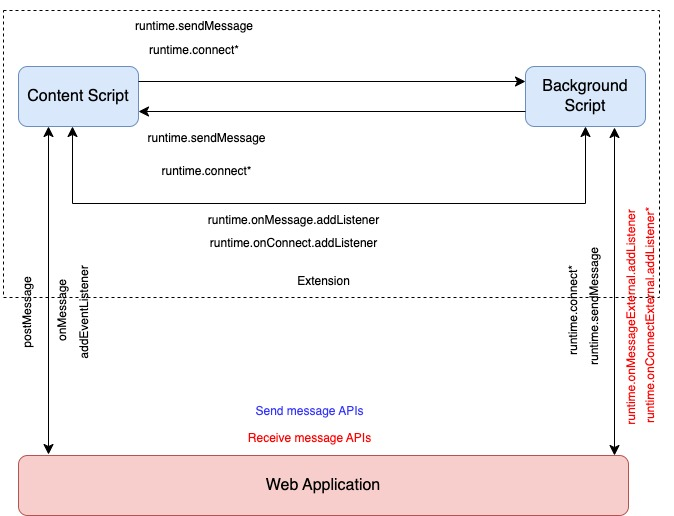
\includegraphics[scale=0.4]{img4.jpg}
		\caption{Data flow in browser extensions}
		\label{img3}
	\end{figure}
\end{frame}

\begin{frame}{Critiques Contd.}
	\begin{itemize}
		\item CACTI does the rate proof generation on clients' Trusted Execution Environment, which can be considered as an overhead because TEE is a very restrictive part of clients machines with limited memory capacity.
		\item A question arises that why should a legitimate client be using its own resources to prove its legitimacy time and again.
		\item Even though this is happening in the background, attackers can exploit client’s resources by accessing TEE.
		\item In the paper, authors have mentioned that there will be two types of list that needs to be stored in the TEE, one is the server-specific list and other would be the global list.
		\item Authors proposed that the name of the server-specific list could be the URL of the website but making the URL as a key in plain text can increase the vulnerability in the system.
	\end{itemize}
\end{frame}


\begin{frame}{Critiques Contd.}
	\begin{itemize}
		\item Any attacker who gains access to the client would easily know for which  website this specific list belongs to and can forge/taper it to cause privacy harm.
		\item This idea of storing plain text URLs makes it easier for the attacker to decode the information about the proposed security system. Our proposed method resolves thing using Hashing with combination to make the system secure. \ref{img2}
		\item The paper suggests using external databases to store protected data for TEEs with limited memory and counters.
	\end{itemize}
\end{frame}

\begin{frame}
	\begin{figure}
		\centering
		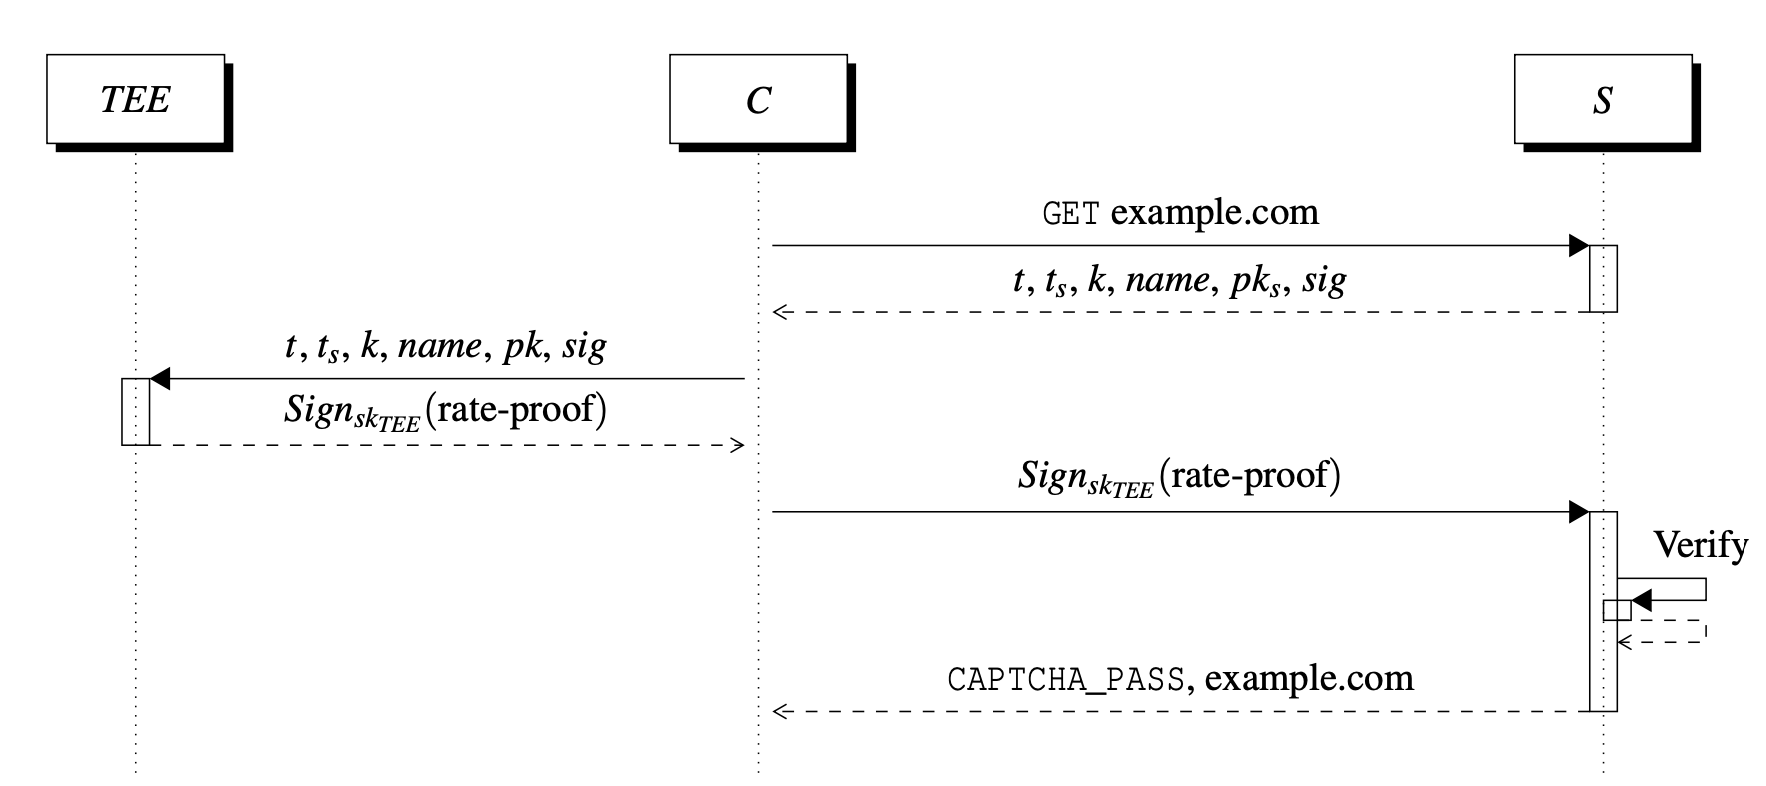
\includegraphics[scale=0.3]{img3.png}
		\caption{Working of CACTI}
		\label{img2}
	\end{figure}
\end{frame}

\begin{frame}{Critiques Contd.}
	\begin{itemize}
		\item Authors provide a method to securely store timestamp data in a standard database, using a chain of hashes to maintain integrity.
		\item The authors propose the idea of Provisioning Authorities responsible for implementing their proposed solution.
		\item However, currently, setting up provisioning authorities is challenging due to the need to coordinate multiple TEE vendors and establish a trusted infrastructure for managing user credentials.
		\item Furthermore, different TEEs have different security protocols, so vendors must share patented information with each other, which can compromise TEE security.
		\item Therefore, establishing a centralized provisioning authority may be difficult and lead to security risks.
	\end{itemize}
\end{frame}




\begin{frame}{References}
	[1] https://en.wikipedia.org/wiki/ReCAPTCHA.

	[2] Gao, Y., Gao, H., Luo, S., Zi, Y., Zhang, S., Mao, W., ... \& Yan, J. (2021, August). Research on the Security of Visual Reasoning CAPTCHA. In USENIX Security Symposium (pp. 3291-3308).

	[3] Hossen, M. I., Tu, Y., Rabby, M. F., Islam, M. N., Cao, H., \& Hei, X. (2020, October). An object detection based solver for google’s image recaptcha v2. In 23rd International Symposium on Research in Attacks, Intrusions and Defenses ({RAID} 2020).

	[4]https://www.fastcompany.com/90369697/googles-new-recaptcha-has-a-dark-side

	[5] Nakatsuka, Y., \& Ozturk, E. (2021, January). CACTI: Captcha avoidance via client-side TEE integration. In 30th USENIX Security Symposium (USENIX Security 21).
\end{frame}

\end{document}
